\subsection{UC-1}
\begin{figure}[H]
    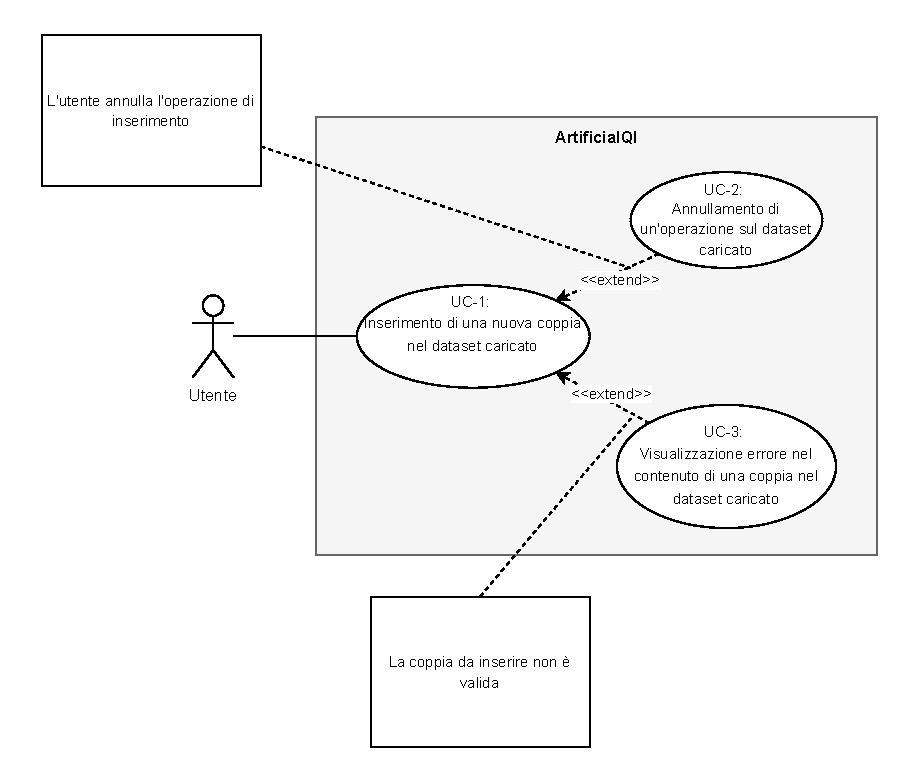
\includegraphics[scale=0.8]{Sezioni/UseCase/Immagini/UC-1.pdf}
    \caption{Diagramma UC-1.}
\end{figure}


\begin{usecase}{UC-1}{Inserimento di una nuova coppia nel dataset corrente}
    
    \req{\hyperref[item:RU-1]{RU-1}} 

    \pre{
        \item Il sistema è attivo e funzionante
        \item Il dataset da modificare è stato caricato come dataset corrente
    }

    \post{
        \item Viene inserita una nuova coppia nel dataset corrente
    }
    
    \actor{Utente}

    \subactors{}

    \trigger{L'utente vuole inserire una nuova coppia nel dataset corrente}
    
    \inc{}

    \base{}

    \scenario{
        \item L'utente richiede l'inserimento di una nuova coppia
        \item L'utente specifica il contenuto per la nuova coppia
        \item L'utente conferma l'inserimento della nuova coppia
        \item La coppia viene inserita nel dataset corrente
    }

    \subscenario{
        \item[2.1] \textbf{L'utente annulla l'operazione di inserimento} 
        \begin{itemize}
            \item[a.] \hyperref[subsec:UC-2]{UC-2}
        \end{itemize}
        \item[3.1] \textbf{La coppia da inserire non è valida}
        \begin{itemize}
            \item[a.] \hyperref[subsec:UC-3]{UC-3}
        \end{itemize}
    }
\end{usecase}


